\documentclass[../main.tex]{subfiles}

\begin{document}
    Der Programcode für Unity wird in C\# geschrieben und im folgenden Kapitel wird auf die Implementation in Unity eingegangen.

    \subsection{Lab 2: Würfel bewegt sich und stösst}
    Alle Kräfte und Berechnungen befinden sich im Code CubeController.cs, welches im Anhang ersichtlich ist.
    Zur Kontrolle der Werte und Grafik Erstellung werden zwei verschiedene CSV Dateien erstellt,
    eine für den elastischen Stoss relevanten Werte und eine für den inelastischen Stoss.

    \begin{figure}[H]
        \begin{center}
            \centerline{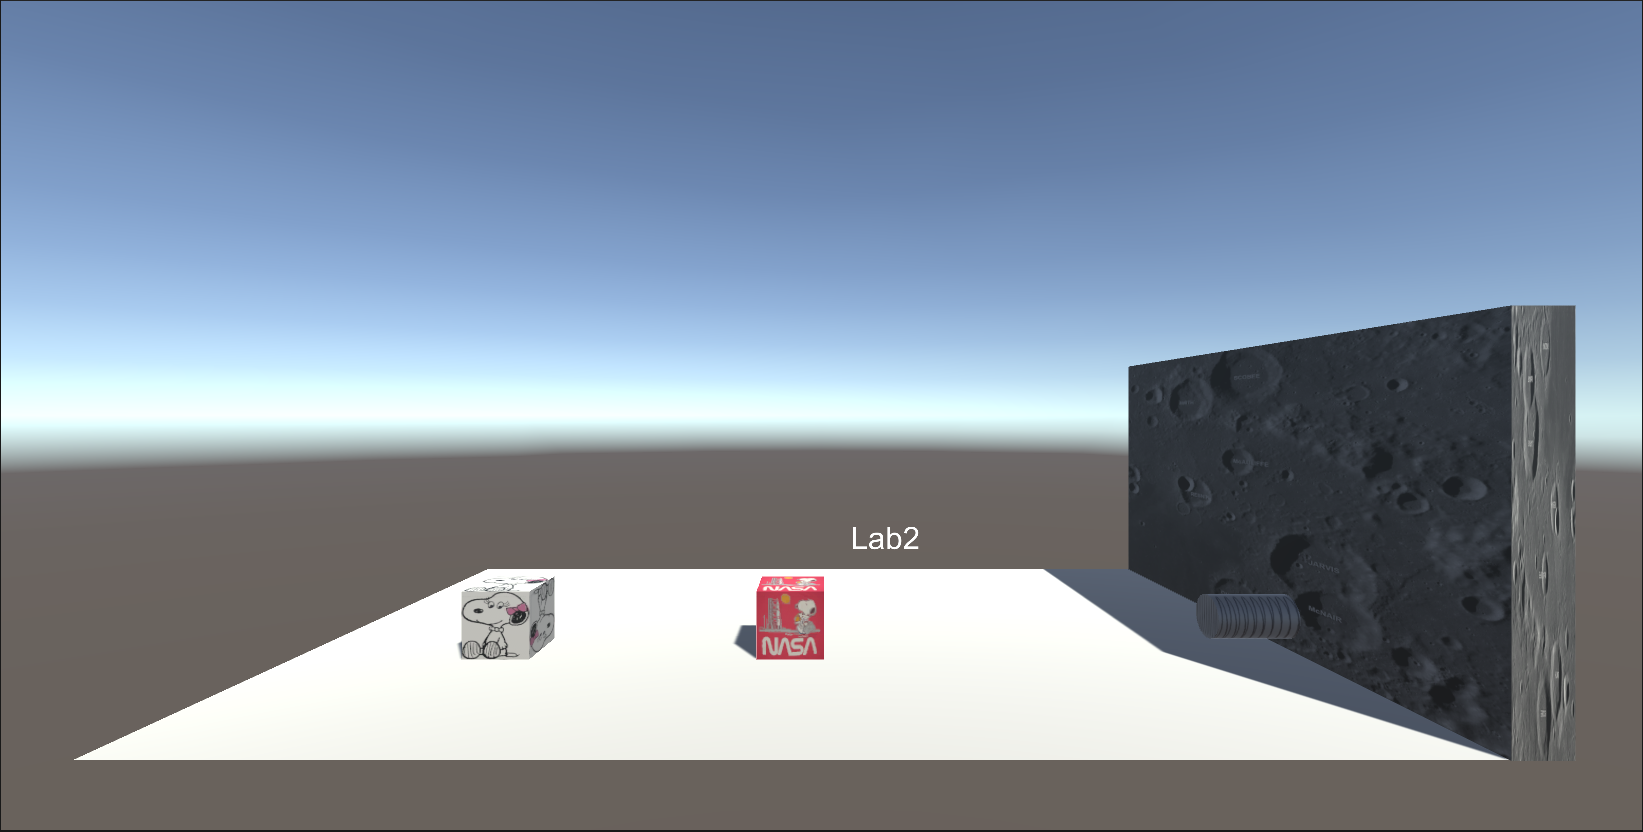
\includegraphics[width=155mm]{./images/2Lab_ExperimentOverview}}
            \caption{Experiment Übersicht}
            \label{fig:2Lab_ExperimentOverview}
        \end{center}
    \end{figure}

    Folgend sind einige wichtige Eigenschaften der Lab relevanten Objekte in Unity aufgelistet:

    \begin{itemize}
        \item Julia:
        \newline Für die Seitenlänge ist die Scale auf 1.5 angepasst, da in Unity beim Würfel eine Seitenlänge von 1 gilt.
        Wichtig ist nicht zu vergessen, das Material auf reibungslos zu ändern, sonst gleiten die Würfel nicht korrekt.
        \begin{figure}[H]
            \begin{center}
                \centerline{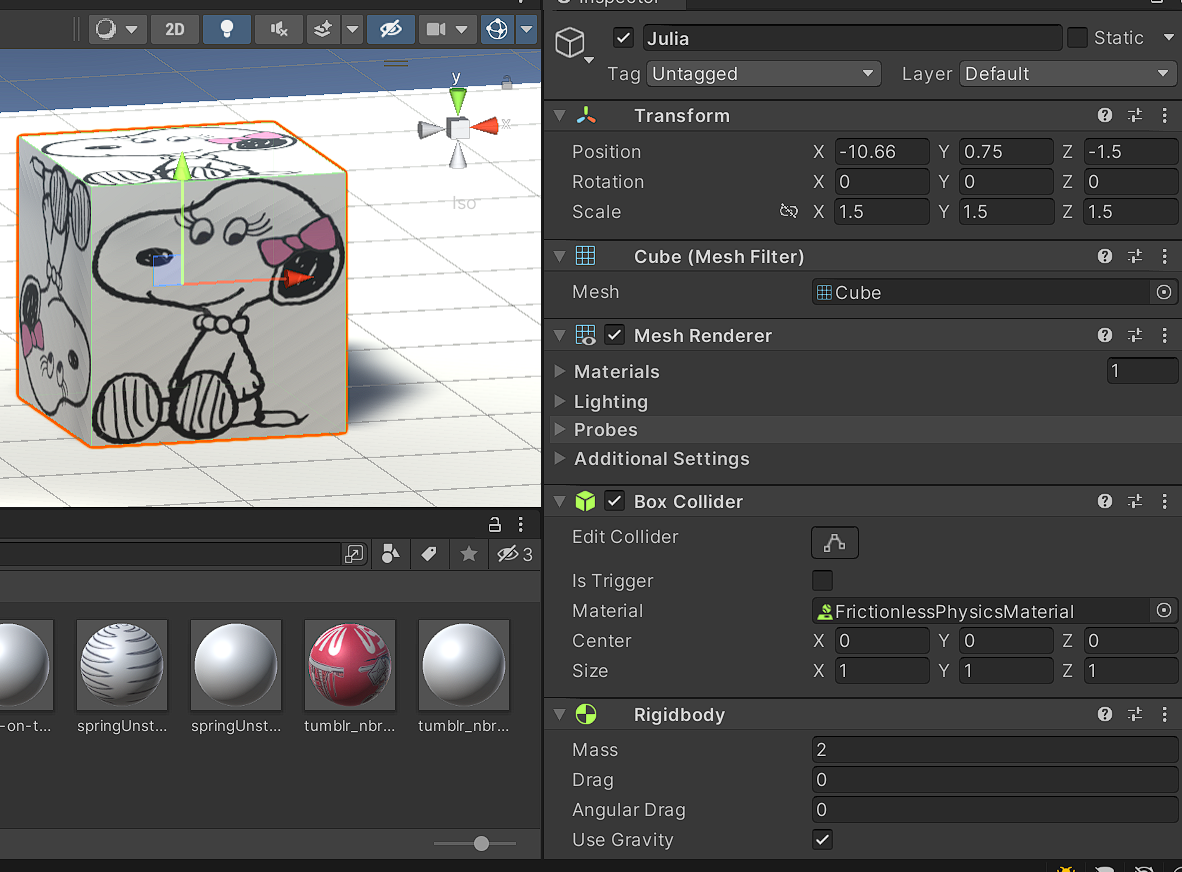
\includegraphics[width=100mm]{./images/2Lab_JuliaCube.PNG}}
                \caption{Einstellung Julia}
                \label{fig:2Lab_JuliaCube}
            \end{center}
        \end{figure}

        \item Romeo:
        \newline Die Eigenschaften sind ausser der Position und Farbe gleich wie bei Julia.
        Romeo besitzt zudem Variabel, über welcher gewisse Parameter an den ihm angehängten Code übergeben werden kann.
        \begin{figure}[H]
            \begin{center}
                \centerline{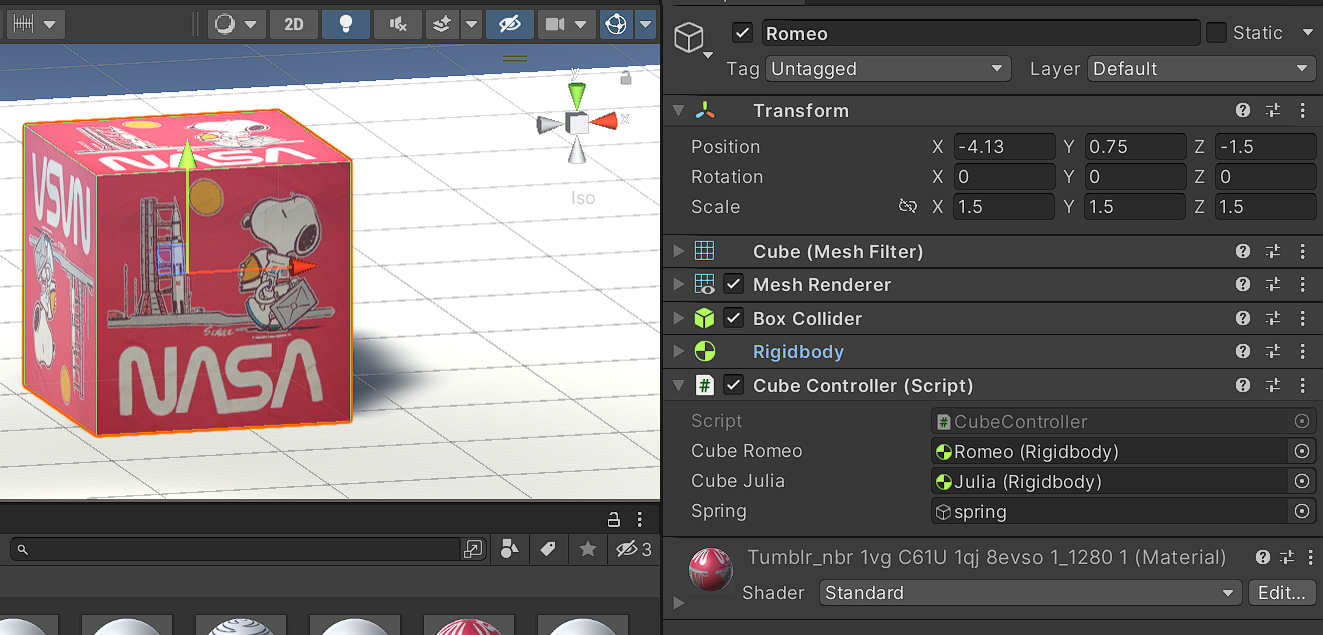
\includegraphics[width=100mm]{./images/2Lab_RomeoCube.PNG}}
                \caption{Einstellung Romeo}
                \label{fig:2Lab_RomeoCube}
            \end{center}
        \end{figure}

        \item Spring:
        \newline Wie in Abbildung \ref{fig:2Lab_RomeoCube} zu sehen ist die Feder nur als GameObject und nicht als Rigdbody
        im Code angegeben. Die Ausrichtung wurde entlang der Y-Achse belassen und um 90 Grad rotiert damit der Zylinder
        liegend erscheint.
        \begin{itemize}
            \item Mesh: Cylinder
            \item Collider direction: Y-Axis
            \begin{figure}[H]
                \begin{center}
                    \centerline{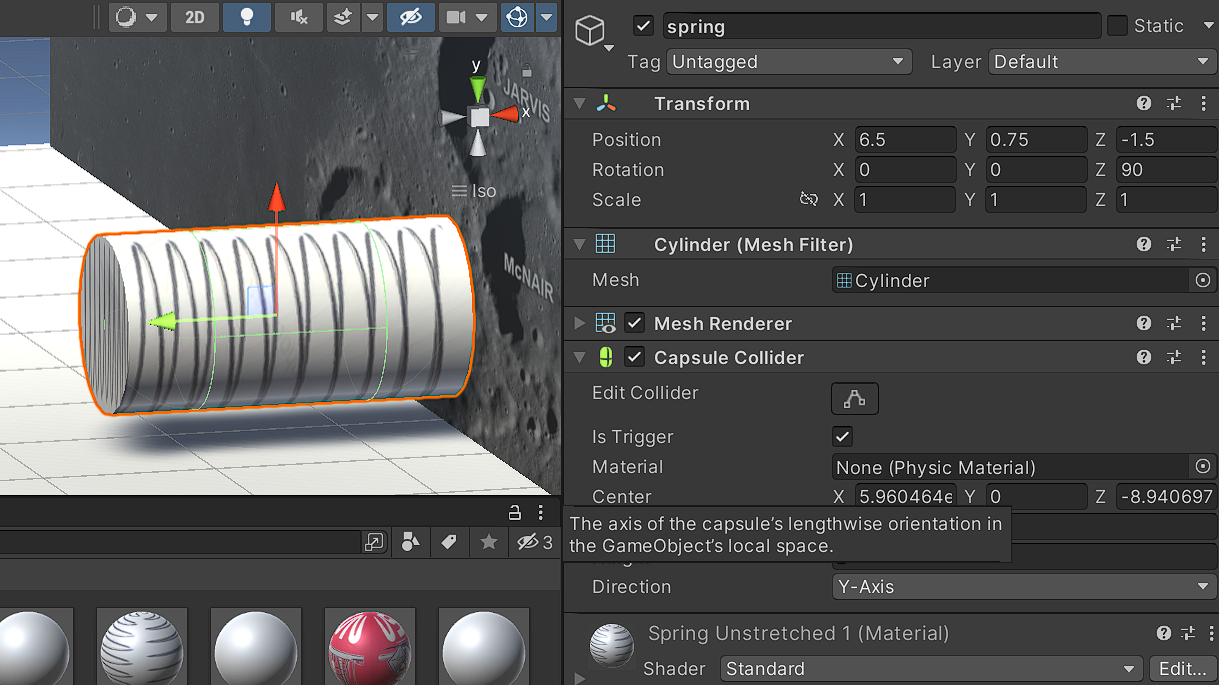
\includegraphics[width=100mm]{./images/2Lab_Spring.PNG}}
                    \caption{Einstellung Feder}
                    \label{fig:2Lab_Spring}
                \end{center}
            \end{figure}
        \end{itemize}

        \item Plane
        \begin{itemize}
            \item Collider Material: FrictionlessPhysicsMaterial
        \end{itemize}
    \end{itemize}
    Da es sich beim CubeController um ein Unity Code handelt, wird von der Klasse Monobeviour geerbt, damit Methoden wie FixedUpdate oder OnCollisionEnter benutzt werden kann.
    Die im vorhinein berechnete konstante Kraft 4, sowie Beschleunigungszeit 1 wird im Code als Konstanten am Anfang deklariert.
    Für die Federauslenkung wird 1.7 gewählt, da die Feder eine Länge von 2 hat und vorher gestoppt werden muss bevor Romeo auf die Wand auftrifft.
    In der Start Methode wird aus den gegebenen Werten die Federkonstante berechnet.

    \begin{lstinputlisting}[label={lst:graphInelastic}, firstline=49, lastline=50]
    {\cubeControllerFiles}
    \end{lstinputlisting}
    Es wird auch die Position ermittelt, welche Romeo zum ersten Mal besitzt, wenn er auf die Feder auftrifft (springMaxDeviation) wie in Abbildung \ref{fig:2Lab_SpringDeviation} rot markiert ist.
    \begin{lstinputlisting}[label={lst:graphInelastic}, firstline=51, lastline=52]
    {\cubeControllerFiles}
    \end{lstinputlisting}


    \begin{figure}[H]
        \begin{center}
            \centerline{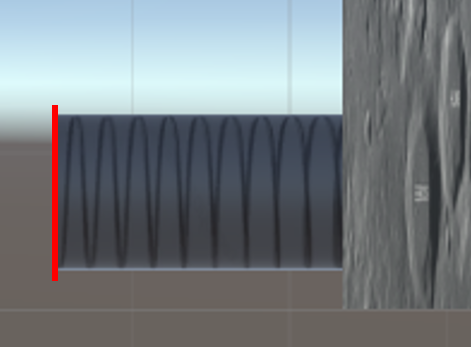
\includegraphics[width=50mm]{./images/2Lab_SpringDeviation.PNG}}
            \caption{Feder mit markierter Berührungspunkt}
            \label{fig:2Lab_SpringDeviation}
        \end{center}
    \end{figure}
    Danach werden die Timeseries Listen deklariert, für die CSV Dateien. Das Hinzufügen der Werte passiert kontinuierlich in der Methode FixedUpdate.
    \newline
    In FixedUpdate gibt es zwei If-Bedingungen. Die erste ist zum Hinzufügen der konstanten Kraft mit der Methode .AddForce bis die Beschleunigunszeit vorüber ist.
    Die zweite If-Bedingung ist zur Überprüfung, ob Romeo die Feder berührt. Dafür muss die Position der rechten Kante von Romeo berechnet werden und mit der
    springMaxDeviation verglichen werden.
    Für den inelastischen Stoss wird die Komponente FixedJoint in der Methode OnCollision implementiert. So bleiben Romeo und Julia  nach ihrer
    Kollision zusammen und gleiten gemeinsam in den Sonnenuntergang.


\end{document}